%%%%%%%%%%%%%%%%%%%%%%%%%%%%%%%%%%%%%%%%%%%%%%%%%%%%%%%%%%%%%%%%%%%%%%%%%%%%%%%%%%%%%%%%%
% 
% Template for Project/Internship reports, for LEEC and LETI at DEE, ISEP,
% by Vitor M. R. Cunha - v1.0, May 2021
% Suggestions and comments are welcomed (vrc at isep dot ipp dot pt).
%
% Template provided as is, NO SUPPORT will be given.
% NO questions related to LaTeX will be answered, go to
% https://ftp.eq.uc.pt/software/TeX/info/lshort/english/lshort.pdf, or search the web.
%
% The DEE document class uses the LaTeX book base class, the original work credits are
% in the document class file.
%
% Overleaf template direct link:
% 
% or go to https://www.overleaf.com/gallery/, and search for: ISEP LEEC
%
%%%%%%%%%%%%%%%%%%%%%%%%%%%%%%%%%% MAIN SETTINGS %%%%%%%%%%%%%%%%%%%%%%%%%%%%%%%%%%%%%%%%

\documentclass[
INFO,			% Use this option to select your DEE degree, options: LEEC, LETI
french,		% Select document language, options: portuguese or english
%draft,			% Uncomment for draft mode (no pictures, no links, overfull hboxes) 
]{DEEclass}

% Use the 'preamble.tex' file (root folder) do add packages and macros. Keep your main.tex file clean.

% FYI, the following packages are preloaded with the document class:
% longtable, xcolor, graphicx, booktabs, caption, csquotes, hyperref,
% calc, listings, datetime2, siunitx, geometry, enumitem

%%%%%%%%%%%%%%%%%%%%%%%%%%%%%%%%%%%%%%%%%%%%%%%%%%%%%%%%%% extra packages
\usepackage{amsmath}		% the principal package in the AMS-LATEX distribution
\usepackage{amsfonts}		% extended set of fonts for use in mathematics
\usepackage{amssymb}		% adds new symbols to be used in math mode
\usepackage{mathrsfs}		% math fonts, e.g., Laplace
\usepackage{float}			% provides the H float modifier option
\usepackage{multirow}		% tables \multirow command
\usepackage{subcaption}		% enables subfigures
\usepackage{lscape}			% for landscape mode
\usepackage{verbatim}		% new verbatim environment, \begin{comment}...\end{comment}, \verbatiminput

%add extra packages if needed here

%%%%%%%%%%%%%%%%%%%%%%%%%%%%%%%%%%%%%%%%%%%%%%%%%%%%%%%%%% temp packages
\usepackage{lipsum}						% for fake text
%\usepackage[textsize=tiny]{todonotes}   % enable To-do notes, use the option "disable" to hide all notes, usage \todo{}

%\usepackage{draftwatermark}			% prints a watermark overlay, uncomment if needed
%\SetWatermarkText{**DRAFT**}
%\SetWatermarkScale{1}
%\SetWatermarkColor[gray]{0.8}

%%%%%%%%%%%%%%%%%%%%%%%%%%%%%%%%%%%%%%%%%%%%%%%%%%%%%%%%%% settings
\AtBeginDocument{					% Rendered PDF metadata:
\hypersetup{pdftitle=\ttitle} 		% Sets the PDF title to your dissertation title
\hypersetup{pdfauthor=\authorname} 	% Sets the PDF author to your name
}

%%%%%%%%%%%%%%%%%%%%%%%%%%%%%%%%%%%%%%%%%%%%%%%%%%%%%%%%%% user defined macros

%....








		 

%%%%%%%%%%%%%%%%%%%%%%%%%%%%%%%% REPORT INFORMATION %%%%%%%%%%%%%%%%%%%%%%%%%%%%%%%%%%%%%

\reporttitle{Titre de votre mémoire} % Your report title

%\reportsubtitle{Com um Subtítulo se Necessário} % and subtitle, uncomment if needed
%\subdate{Janeiro, 2021} % Uncomment for a static submission date, or leave it as a comment for automatic date (month+year) 

\author{Prénom NOM}	% Your name
\studentnumber{NNNNNNNN}	% Your student number
\studentemail{prenom.nom.etu@univ-lille.fr}	% Your student email address  

\advisor{Prénom NOM de l'encadrant}{prenom.nom@univ-lille.fr}	% Your advisor name and email
%\coadvisor{Nom du co-encadrant}{xxx.yyy@univ-lille.fr}	% Your co-advisor name and email, comment this line if not needed
% \company{Université de Lille}	% The company name where you developed your work, comment this line if not needed

%%%%%%%%%%%%%%%%%%%%%%%%%%%%% USER DEFINED LISTS %%%%%%%%%%%%%%%%%%%%%%%%%%%%%%%%%%%%%%%%
\makeglossaries						% Consider the following files in the 'front' folder:
%----------------------------------------------------------------------------------------
%	GLOSSARY
%----------------------------------------------------------------------------------------

% Only the used entries will be displayed in the printed list, ie, you need to used a term at least once
% In italic if not in the main document language

% terms definition usage:
% \newglossaryentry{<tag>}{name={<term>},description={<description of the term>}}

\newglossaryentry{gloss}{
name={glossaire}, 
description={est une liste alphabétique des termes d'un domaine de connaissance donné avec la définition de ces mêmes termes.},
}

\newglossaryentry{pack}{
name={\textit{package}}, 
description={est un fichier ou un ensemble de fichiers contenant des commandes \LaTeX{} supplémentaires qui ajoutent de nouvelles fonctionnalités de style ou modifient celles existantes.},
sort={package}	%needed for sorting when using LaTeX commands in the 'name' field
}

\newglossaryentry{lipsum}{
name={\textit{Lorem Ipsum}}, 
description={est une séquence de mots, généralement latins, utilisée pour remplir l'espace de texte dans une publication, afin de tester les options de mise en forme et d'édition et la disposition des éléments graphiques avant l'insertion du contenu.},
sort={Lorem Ipsum}
}
			% Edit to define your glossary entries list
%----------------------------------------------------------------------------------------
%	ACRONYMS LIST
%----------------------------------------------------------------------------------------

% Only the used entries will be displayed in the printed list, ie, you need to used a acronym at least once
% Full name in italic if not in the main document language

%acronym definition usage:
%\newacronym{<tag>}{<acronym>}{<full name>}

\newacronym{wys}{WYSIWYG}{\textit{What You See Is What You Get}}
\newacronym{fil}{FIL}{Formations en Informatique de Lille}
\newacronym{api}{API}{\textit{Application Programming Interface}}
\newacronym{ascii}{ASCII}{\textit{American Standard Code for Information Interchange}}
\newacronym{html}{HTML}{\textit{HyperText Markup Language}}
\newacronym{fst}{FST}{Faculté des Sciences et Technologies}
\newacronym{info}{INFO}{Master mention Informatique}
\newacronym{miage}{MIAGE}{Master mention MIAGE}
\newacronym{usb}{USB}{\textit{Universal Serial Bus}}
\newacronym{pdf}{PDF}{\textit{Portable Document Format}}
			% Edit to define your acronyms entries list
%----------------------------------------------------------------------------------------
%	SYMBOLS LIST
%----------------------------------------------------------------------------------------

% terms definition usage:
% \newglossaryentry{<tag>}{
% name={<symbol>},
% sort={<text for the alphabetical sorting>},
% description={<description of the symbol>},
% unit={<units to display>},
% type=symbolslist}

\newglossaryentry{f}{
name={\ensuremath{f}},
sort={f},
description={force},
unit=\si{\newton},
type=symbolslist}

\newglossaryentry{i}{
name={\ensuremath{i}},
sort={i},
description={courant},
unit=\si{\ampere},
type=symbolslist}

\newglossaryentry{m}{
name=\ensuremath{M},
sort={m},
description={masse},
unit=\si{\kilogram},
type=symbolslist}

\newglossaryentry{p}{
name=\ensuremath{P},
sort={p},
description={puissance},
unit=\si{\watt},
type=symbolslist}

\newglossaryentry{theta}{
name=\ensuremath{\theta},
sort={z1},
description={déplacement angulaire},
unit=\si{\radian},
type=symbolslist}

\newglossaryentry{omega}{
name=\ensuremath{\omega},
sort={z2},
description={vitesse angulaire},
unit=\si{\radian\per\second},
type=symbolslist}

\newglossaryentry{x}{
name=\ensuremath{x},
sort={x},
description={déplacement},
unit=\si{\meter},
type=symbolslist}

% Greek: alpha,beta,gamma,delta,epsilon,zeta,eta,theta,iota,kappa,lambda,mu,nu,xi,omikron,pi,rho,sigma,tau,upsilon,phi,chi,psi,omega
				% Edit to define your symbols entries list

%%%%%%%%%%%%%%%%%%%%%%%%%%%%%%%%%%%%%%%%%%%%%%%%%%%%%%%%%%%%%%%%%%%%%%%%%%%%%%%%%%%%%%%%%
\begin{document}
\frontmatter

%----------------------------------------------------------------------------------------
%	TITLE PAGES
%----------------------------------------------------------------------------------------
\pagestyle{plain} % Default to the plain heading style until the thesis style is called for the body content
\printcoverpage
\printaftercoverpage
\cleardoublepage















%%%%%%%%%%%%%%%%%%%%%%%%%%%%%%%%%%% FRONTMATTER %%%%%%%%%%%%%%%%%%%%%%%%%%%%%%%%%%%%%%%%%
% Consider the following front matter sections provided as separate files in the 'front' folder.
% Comment the lines regarding the sections you will not use, or edit the file contents as needed

%%----------------------------------------------------------------------------------------
%	DEDICATION
%----------------------------------------------------------------------------------------

\dedicatory{
(Facultatif) Vous pouvez utiliser cette section pour dédier votre travail à quelqu'un\ldots
} 
		% Edit if you want to dedicate your work to someone, or comment this line if not used
%%----------------------------------------------------------------------------------------
%	ACKNOWLEDGEMENTS
%----------------------------------------------------------------------------------------

\begin{acknowledgements}

(Facultatif) Remerciements dus\ldots

\end{acknowledgements}
	% Edit to add the due acknowledgements, or comment this line if not used
%----------------------------------------------------------------------------------------
%	ABSTRACT PAGES
%----------------------------------------------------------------------------------------

% IMPORTANT NOTE: the abstract must always be written in two languages. If the report
% is written in Portuguese you have selected 'portuguese' as the language in the document class.
% Therefore, the portuguese version of the abstract must come first, so write it in the
% below area denoted by 'MAIN LANGUAGE ABSTRACT'. The english version follows in the
% 'SECOND LANGUAGE ABSTRACT' section.
% If the report is written in English, first will come the abstract in English
% ('MAIN LANGUAGE ABSTRACT') and then in Portuguese ('SECOND LANGUAGE ABSTRACT').

\begin{abstract}
%%%%%%%%%%%%%%%%%%%%%%%%%%%%%% MAIN LANGUAGE ABSTRACT %%%%%%%%%%%%%%%%%%%%%%%%%%%%%%%%%%

Ici, le résumé de tous les travaux réalisés doit être présenté. Cette section ne doit pas dépasser une page.

Vous devez contextualiser le problème que vous souhaitez résoudre ou l'hypothèse que vous allez formuler, essayer de mettre en évidence les avantages et les inconvénients (le cas échéant) de la solution trouvée, ainsi que la manière dont la solution/hypothèse a été validée. Dans ce dernier point, il doit se référer aux développements réalisés, et à la manière dont il a validé (conformité) et évalué (performance) la solution trouvée.

Le document doit toujours contenir deux versions du résumé: une première dans la langue du texte principal et la seconde dans une autre langue. Ce \textit{template} suppose que les deux langues considérées sont toujours le portugais et l'anglais, donc la classe placera les en-têtes respectifs en fonction de la langue sélectionnée dans les options de classe dans le fichier \file{main.tex}.

%----------------------------------------------------------------------------------------

\vspace*{10mm} 
\noindent
\textbf{\keywordslabel}: Liste, séparés par des virgules, des mots, des phrases ou des acronymes clés dans le cadre des travaux décrits dans ce texte.

%%%%%%%%%%%%%%%%%%%%%%%%% END OF THE MAIN LANGUAGE ABSTRACT %%%%%%%%%%%%%%%%%%%%%%%%%%%%%%
\end{abstract}
\begin{secondlangabstract}
%%%%%%%%%%%%%%%%%%%%%%%%%%%%%% SECOND LANGUAGE ABSTRACT %%%%%%%%%%%%%%%%%%%%%%%%%%%%%%%%%%

The summary of all the developed work should be presented here. This section should not exceed one page.

Start the abstract with the contextualization of the problem you intend to solve or the hypothesis you will formulate. Try to highlight the advantages and disadvantages (if any) of the solution found, as well as the way in which the solution/hypothesis was validated. In this last point, you should refer to the developments made, and to the way you validated (compliance) and evaluated (performance) the solution found.

The document must always contain two versions of the abstract: a first in the language of the main text and the second one in another language. This template assumes that the two languages are always Portuguese and English, therefore, the class will place the correct section headers according to the language selected in the class options in the \file{main.tex} file.


%----------------------------------------------------------------------------------------

\vspace*{10mm} 
\noindent
\textbf{\keywordslabel}: Comma separated list of words, phrases, or key acronyms within the scope of your developed work. 

%%%%%%%%%%%%%%%%%%%%%%%%%% END OF THE SECOND LANGUAGE ABSTRACT %%%%%%%%%%%%%%%%%%%%%%%%%%%%%
\end{secondlangabstract}

			% Edit the file to write the document Abstract. Two languages are always required.
%----------------------------------------------------------------------------------------
%	FONTMATTER LISTS
%----------------------------------------------------------------------------------------
\pdfbookmark[0]{\contentsname}{toc}
\tableofcontents 	
\glsresetall
%----------------------------------------------------------------------------------------

% Of the following lists, comment the ones you will not use in your document

\listoffigures 			% Prints the list of figures

\listoftables 			% Prints the list of tables

\printlistoflistings	% Prints the list of listings (source code segments)

\printlistofterms		% Prints the list of USED terms (glossary)

\printlistofacronyms{XXXXXXXXI} % Prints the list of USED acronyms
% Change the argument with random letters to adjust the left alignment of the acronyms full name column

\printlistofsymbols		% Prints the list of ALL defined symbols
	% Edit the file to select the lists to be shown (figures, tables, source code segments, glossary, acronyms, symbols)

%%%%%%%%%%%%%%%%%%%%%%%%%%%%%%%%%%% MAINMATTER %%%%%%%%%%%%%%%%%%%%%%%%%%%%%%%%%%%%%%%%%
\mainmatter 
\pagestyle{thesis} 				

% Include the chapters of the document as separate files from the 'chapters' folder

%%%%%%%%%%%%%%%%%%%%%%%%%%%%%%%%%%%% Chapter Template

\chapter{Introduction} 	% Main chapter title
\label{Chapter1} 		% For referencing the chapter elsewhere, usage \ref{Chapter1}

%%%%%%%%%%%%%%%%%%%%%%%%%%%%%%%%%%%%
Ce document vise à guider l'étudiant dans l'élaboration de son mémoire de Master.

L'auteur doit tenir compte des règles générales suivantes lors de la préparation du document:
\begin{itemize}
    \item Il est essentiel de réfléchir, avant d'écrire, à la substance de ce qui est destiné à être transmis;
    \item Vous devez organiser le texte en évitant sa division excessive en sujets qui sont censés tomber sous le thème principal de la section à laquelle ils appartiennent. Une spécialisation excessive peut révéler un manque de connaissances et/ou de réflexion. En ce sens, vous devez, avant de commencer à écrire, travailler à affiner l'organisation du texte afin d'éviter qu'il y ait plus de 2 niveaux de ``profondeur'' dans chaque section (respectivement, sous-section et sous-sous-sous-section). Notez que le nombre de chapitres, sections et sous-sections de ce document n'est pas contraignant ni même indicatif, il ne sert qu'à ses fins;
    \item Le document doit être rédigé en français ou en anglais dans un style approprié (éviter le ton familier, les lieux communs et les mots à la mode) et correct d'un point de vue grammatical (que ce soit d'un point de vue syntaxique ou sémantique);
    \item Soyez particulièrement prudent avec l'utilisation des adjectifs (ils conduisent facilement à l'exagération), des adverbes (rien, ou presque rien, ajoutent-ils) et des signes de ponctuation (surtout l'utilisation correcte des virgules);
    \item Le style adopté pour l'écriture doit être conforme aux exigences d'un travail scientifique trouvé dans les publications imprimées;
    \item D'une manière générique, vous devriez utiliser la 3ème personne du singulier (éventuellement du pluriel), sauf pour les endroits où c'est clairement déplacé, par exemple, dans la section de remerciements;
    \item Utilisez le style \textit{italic} chaque fois que des termes sont utilisés dans des langues autres que la langue adoptée dans le rapport;
    \item L'utilisation d'acronymes implique que la première fois qu'ils sont utilisés, ils doivent être présentés en entier, en mettant entre parenthèses l'acronyme respectif qui sera utilisé. Cependant, il est toujours possible, plus tard dans le texte, et dans un souci de lisibilité, de répéter le sens de l'acronyme. Tous les acronymes doivent être présentés par ordre alphabétique dans la section ``Liste des acronymes'';
    \item L'utilisation correcte des unités, de leurs multiples et sous-multiples;
    \item Les images et les tableaux doivent, en principe, apparaître en haut ou en bas de la page. Les légendes apparaissent immédiatement après les chiffres et les listes. Dans le cas des tableaux, les légendes les précèdent;
    \item Toutes les figures, tableaux et autres listes doivent être mentionnés dans le texte afin qu'ils soient encadrés dans les idées transmises par l'auteur. Cette référence, en règle générale, doit être faite avant l'apparition de la figure, du tableau ou de la liste;
    \item Il doit indiquer tout au long du texte les références documentaires utilisées, notamment dans les citations (pures ou littérales), marquées de l'utilisation de guillemets, ainsi qu'en cas de réutilisation de graphiques, figures, tableaux, formules, etc., d’autres sources.
\end{itemize}

Plus précisément, dans ce premier chapitre obligatoire (``Introduction''), l'auteur doit:
\begin{itemize}
    \item contextualiser la proposition de travail au sein de l'entreprise, à partir d'un autre travail déjà réalisé, d'un point de vue scientifique et/ou technologique, etc.,
    \item présente clairement les objectifs qu'il se propose d'atteindre,
    \item décrivent succinctement, mais objectivement, la solution ou l'hypothèse recommandée,
    \item présente brièvement mais clairement les développements réalisés,
    \item identifie comment la solution trouvée a été validée et évaluée,
    \item décrivent l'organisation du document.
\end{itemize}

Sans nécessiter d'organisation particulière pour ce chapitre, 4 sections (avec le texte \gls{lipsum}) sont indiquées à titre d'exemple, qui peuvent être incorporées dans cette partie du document: Contextualisation, Description du projet, Calendrier et Organisation du rapport.
%%%%%%%%%%%%%%%%%%%%%%%%%%%%%%%%%%%% SECTION 1

\section{Contextualisation}
\label{sec:Ch1.1}

\lipsum[1] % inserts fake text, to be removed in your dissertation

%%%%%%%%%%%%%%%%%%%%%%%%%%%%%%%%%%%% SECTION 2

\section{Description du projet}
\label{sec:Ch1.2}

\lipsum[2]

%%%%%%%%%%%%%%%%%%%%%%%%%%%%%%%%%%%% SUBSECTION 1

\subsection{Objectifs}
\label{sub:Ch1.2.1}

\lipsum[2]

%%%%%%%%%%%%%%%%%%%%%%%%%%%%%%%%%%%% SECTION 3

\section{Calendrier}
\label{sec:Ch1.3}

\lipsum[1]
% you could use the pgfgantt package: https://ctan.org/pkg/pgfgantt


%%%%%%%%%%%%%%%%%%%%%%%%%%%%%%%%%%%% SECTION 4

\section{Organisation du rapport}
\label{sec:Ch1.4}

\lipsum[2]


% Chapter 2

\chapter{Comment utiliser le \textit{template} \LaTeX{} pour les mémoires}	%The main chapter title
\chaptermark{O \textit{Template}}	%Short version for page header. Comment if not needed
\label{Chapter2}	%For referencing the chapter elsewhere, use \ref{Chapter2} 

%%%%%%%%%%%%%%%%%%%%%%%%%%%%%%%%%%%%

L'option de \LaTeX{} pour préparer le rapport favorise l'aspect graphique du document final, mais un document visuellement beau ne remplace pas une rédaction soignée et une présentation structurée des idées. Ce chapitre est dédié à la présentation du \textit{template} et à certains aspects de l'insertion de citations, figures, tableaux, équations et autres éléments dont la mise en forme doit être cohérente dans tout le document.

Le \textit{template} \LaTeX{} pour les mémoires de Master a été développé, et est maintenu par Romain Rouvoy, sur la base de la \textit{template} `` Master / Doctor Thesis '' disponible sur \url{www.LaTeXTemplates.com}. Les suggestions et commentaires peuvent être envoyés à \verb|romain.rouvoy@univ-lille.fr|. Cependant, il convient de noter que \underline{o \textit{template} est fourni sans assistance} et que l'utilisateur est entièrement responsable de toute modification du code et/ou des fichiers fournis.

\begin{comment}
L'environnement de commentaire est utilisé pour commenter facilement de grandes sections de code LateX. L'environnement de commentaire est utilisé pour commenter facilement de grandes sections de code LateX. L'environnement de commentaire est utilisé pour commenter facilement de grandes sections de code LateX. L'environnement de commentaire est utilisé pour commenter facilement de grandes sections de code LateX. L'environnement de commentaire est utilisé pour commenter facilement de grandes sections de code LateX.
\end{comment}

%%%%%%%%%%%%%%%%%%%%%%%%%%%%%%%%%%%%

\section{Introduction à \LaTeX{}}
\label{sec:Ch2.1}

\LaTeX{} est un outil puissant pour produire des documents. Contrairement aux traitements de texte courants comme Microsoft Word ou LibreOffice Writer, \LaTeX{} n'est pas un programme \ac{wys}. Au lieu de cela, un document écrit pour \LaTeX{} est en fait un simple fichier texte sans aucun formatage. Tout format requis dans le document final est défini par des commandes spécifiques que \LaTeX{} interprète lors de la compilation du document. Par exemple, pour mettre un mot en italique, dans le fichier de code, vous écrivez \verb|\textit{mot}| pour obtenir \textit{mot} dans le document final. Cela signifie que \LaTeX{} est un langage \emph{balisage}, similaire à \ac{html}. De cette manière, l'auteur peut se concentrer sur la tâche essentielle de l'écriture, sans avoir à se soucier de la mise en forme, de la pagination et des autres arrangements visuels du document en préparation. \LaTeX{} est largement utilisé dans le milieu universitaire pour la préparation et la publication de documents scientifiques dans plusieurs domaines, notamment les mathématiques, les statistiques, l'ingénierie, la physique, l'économie, entre autres. Il joue également un rôle important dans la préparation et la publication de livres.

Pour ceux qui commencent par \LaTeX{}, en plus des nombreux \textit{sites Web} contenant des informations (par exemple, \url{www.overleaf.com/learn}), le livre gratuit intitulé ``One no such a small introduction to \LaTeX{}'' disponible en plusieurs langues sur \url{www.ctan.org/tex-archive/info/lshort/}.

%%%%%%%%%%%%%%%%%%%%%%%%%%%%%%%%%%%%

\section{Comment utiliser le modèle}

Le \textit{template} est disponible et prêt à être utilisé dans Moodle et dans la \textit{Overleaf Templates Gallery}. Indépendamment du choix de développer votre rapport sur Overleaf ou localement sur votre ordinateur personnel, il est essentiel de se familiariser avec la structure des répertoires et des fichiers fournis avec \textit{template}.

\paragraph{Répertoires}

Les noms de répertoires sont généralement explicites:
\begin{itemize}
     \item \textbf{chapitres} - ce répertoire est l'endroit où vous devez placer les chapitres du rapport, y compris les pièces jointes. Chaque chapitre (et annexe) doit avoir son propre fichier \file{.tex} et, bien qu'il n'y ait pas de règle stricte pour le nom et le nombre de chapitres, il doit toujours y avoir une ``Introduction'' et les ``Conclusions'';

     \item \textbf{figures} - ce répertoire doit contenir toutes les figures utilisées dans le rapport. Il est recommandé d'utiliser un système de noms de fichiers qui facilite l'association d'un fichier avec une section du document;

     \item \textbf{front} - ce répertoire contient déjà plusieurs fichiers pour les sections initiales prédéfinies du rapport, appelées \textit{frontmatter}. Vous pouvez choisir de ne pas utiliser certaines de ces sections si elles ne concernent pas votre document.
\end{itemize}

\paragraph{Fichiers}
En plus de la structure des répertoires, plusieurs fichiers sont également fournis, la plupart en texte brut et dont le contenu peut être visualisé avec un éditeur de texte. Après la compilation avec \LaTeX{} plusieurs fichiers auxiliaires sont créés automatiquement, cependant, en règle générale, vous n'avez pas besoin de les prendre en compte.

\begin{itemize}
    \item \textbf{sampleRefs.bib} - c'est le fichier pour BibTeX qui contient toutes les références que vous citerez dans le rapport. Cela peut être modifié manuellement, mais il existe des programmes disponibles (par exemple, \url{www.jabref.org}) pour gérer les références qui facilitent l'ensemble du processus. Vous pouvez renommer le fichier tant que cette modification est également effectuée dans le fichier \file{main.tex}. Les références seront présentées dans le document final dans le style \textbf{ieeetr}. Considérez les exemples de divers types de références fournis dans le fichier \file{sampleRefs.bib} pour créer votre propre liste;

    \item \textbf{DEEclass.cls} - ce fichier définit la classe de document DEEclass. Il est fortement déconseillé de sa modification;

    \item \textbf{preamble.tex} - ce fichier doit être utilisé pour ajouter \glspl{pack}, des paramètres et des macros, spécifiques à votre document. Cela évite que le préambule du fichier principal \file{main.tex} ne devienne trop long;

    \item \textbf{main.tex} - c'est le fichier le plus important pour définir votre document. Le code de ce fichier définit la structure et contient les instructions qui conduisent \LaTeX{} à générer le PDF final. Tenez compte des commentaires présentés dans le fichier lui-même afin de savoir ce que fait chaque ligne / section de code et comment \textit{template} peut être adapté à votre cas. C'est ce fichier que vous devez éditer pour démarrer la préparation de votre rapport. Félicitations pour avoir décidé d'utiliser \LaTeX{}!
\end{itemize}

%%%%%%%%%%%%%%%%%%%%%%%%%%%%%%%%%%%%

\paragraph{Modification du fichier \file{main.tex}}
\label{subsec: Ch2.2.3}

Pour démarrer votre document, la première chose à faire est de renseigner vos informations et de choisir certaines options dans le fichier \file{main.tex}. Après avoir ouvert ce fichier, recherchez la section identifiée comme `` PARAMÈTRES PRINCIPAUX '' (ligne 18). Dans cette section, vous devez choisir votre mention, parmi les deux options:
\begin{itemize}
    \item \acs{info} (\acl{info})
    \item \acs{miage} (\acl{miage})
\end{itemize}
\newpage
\noindent et la langue principale du document, des deux options:
\begin{itemize}
    \item french
    \item english
\end{itemize}

Lorsque vous choisissez le français comme langue principale, l'anglais est automatiquement utilisé comme deuxième langue. Le contraire est vrai si vous choisissez l'anglais comme langue principale du document.

Pour procéder à la personnalisation, retrouvez la section `` INFORMATIONS DE RAPPORT '' (ligne 29). Après avoir rempli les champs de cette section avec les données:
\begin{itemize}
    \item titre du poste (et sous-titre si nécessaire),
    \item identification du candidat (nom, numéro mécanographique et \textit{email}),
    \item identification de l'élément de l'encadrant \ac{fil} (nom et \textit{email}),
    \item le cas échéant, identification du co-superviseur de \ac{fil} (nom et \textit{email}),
    \item le cas échéant, identification de l'entreprise où s'est déroulé le stage (nom) et du conseiller (nom et \textit{email}),
\end{itemize}

\noindent peut compiler votre document. Toutes les informations saisies doivent maintenant être visibles (sur les pages de garde) dans le PDF généré.

Le fichier \file{main.tex} est également utilisé pour définir la structure et le contenu du rapport. Tenez compte des commentaires que vous pouvez lire tout au long du fichier pour savoir où placer, par exemple, de nouveaux chapitres ou masquer des sections que vous n'avez pas l'intention d'utiliser dans votre document (par exemple, `` Dédicace ''). Brièvement dans la rubrique `` FRONTMATTER '' (ligne 55):

\begin{itemize}
    \item La ligne \verb|%----------------------------------------------------------------------------------------
%	DEDICATION
%----------------------------------------------------------------------------------------

\dedicatory{
(Facultatif) Vous pouvez utiliser cette section pour dédier votre travail à quelqu'un\ldots
} 
| fait référence à la section ``Dédicace''. Si vous souhaitez rédiger une dédicace, modifiez le fichier \path{/front/1_dedicatory.tex}. Sinon, commentez simplement la ligne pour que le contenu du fichier ne soit pas pris en compte;
    \item La ligne \verb|%----------------------------------------------------------------------------------------
%	ACKNOWLEDGEMENTS
%----------------------------------------------------------------------------------------

\begin{acknowledgements}

(Facultatif) Remerciements dus\ldots

\end{acknowledgements}
| reportez-vous à la section ``Remerciements'' et pour le modifier, allez dans le fichier \path{/front/2_acknowledgements.tex};
    \item La ligne \verb|%----------------------------------------------------------------------------------------
%	ABSTRACT PAGES
%----------------------------------------------------------------------------------------

% IMPORTANT NOTE: the abstract must always be written in two languages. If the report
% is written in Portuguese you have selected 'portuguese' as the language in the document class.
% Therefore, the portuguese version of the abstract must come first, so write it in the
% below area denoted by 'MAIN LANGUAGE ABSTRACT'. The english version follows in the
% 'SECOND LANGUAGE ABSTRACT' section.
% If the report is written in English, first will come the abstract in English
% ('MAIN LANGUAGE ABSTRACT') and then in Portuguese ('SECOND LANGUAGE ABSTRACT').

\begin{abstract}
%%%%%%%%%%%%%%%%%%%%%%%%%%%%%% MAIN LANGUAGE ABSTRACT %%%%%%%%%%%%%%%%%%%%%%%%%%%%%%%%%%

Ici, le résumé de tous les travaux réalisés doit être présenté. Cette section ne doit pas dépasser une page.

Vous devez contextualiser le problème que vous souhaitez résoudre ou l'hypothèse que vous allez formuler, essayer de mettre en évidence les avantages et les inconvénients (le cas échéant) de la solution trouvée, ainsi que la manière dont la solution/hypothèse a été validée. Dans ce dernier point, il doit se référer aux développements réalisés, et à la manière dont il a validé (conformité) et évalué (performance) la solution trouvée.

Le document doit toujours contenir deux versions du résumé: une première dans la langue du texte principal et la seconde dans une autre langue. Ce \textit{template} suppose que les deux langues considérées sont toujours le portugais et l'anglais, donc la classe placera les en-têtes respectifs en fonction de la langue sélectionnée dans les options de classe dans le fichier \file{main.tex}.

%----------------------------------------------------------------------------------------

\vspace*{10mm} 
\noindent
\textbf{\keywordslabel}: Liste, séparés par des virgules, des mots, des phrases ou des acronymes clés dans le cadre des travaux décrits dans ce texte.

%%%%%%%%%%%%%%%%%%%%%%%%% END OF THE MAIN LANGUAGE ABSTRACT %%%%%%%%%%%%%%%%%%%%%%%%%%%%%%
\end{abstract}
\begin{secondlangabstract}
%%%%%%%%%%%%%%%%%%%%%%%%%%%%%% SECOND LANGUAGE ABSTRACT %%%%%%%%%%%%%%%%%%%%%%%%%%%%%%%%%%

The summary of all the developed work should be presented here. This section should not exceed one page.

Start the abstract with the contextualization of the problem you intend to solve or the hypothesis you will formulate. Try to highlight the advantages and disadvantages (if any) of the solution found, as well as the way in which the solution/hypothesis was validated. In this last point, you should refer to the developments made, and to the way you validated (compliance) and evaluated (performance) the solution found.

The document must always contain two versions of the abstract: a first in the language of the main text and the second one in another language. This template assumes that the two languages are always Portuguese and English, therefore, the class will place the correct section headers according to the language selected in the class options in the \file{main.tex} file.


%----------------------------------------------------------------------------------------

\vspace*{10mm} 
\noindent
\textbf{\keywordslabel}: Comma separated list of words, phrases, or key acronyms within the scope of your developed work. 

%%%%%%%%%%%%%%%%%%%%%%%%%% END OF THE SECOND LANGUAGE ABSTRACT %%%%%%%%%%%%%%%%%%%%%%%%%%%%%
\end{secondlangabstract}

| fait référence aux sections ``Résumé'' et ``Abstract'', et leur contenu est modifié dans le fichier \path{/front/3_abstract.tex}. Notez que vous devrez toujours rédiger cette section en deux langues, lisez attentivement les instructions contenues dans le fichier. C'est dans cette section que sont également introduits les mots-clés associés à votre travail;
    \item La ligne \verb|%----------------------------------------------------------------------------------------
%	FONTMATTER LISTS
%----------------------------------------------------------------------------------------
\pdfbookmark[0]{\contentsname}{toc}
\tableofcontents 	
\glsresetall
%----------------------------------------------------------------------------------------

% Of the following lists, comment the ones you will not use in your document

\listoffigures 			% Prints the list of figures

\listoftables 			% Prints the list of tables

\printlistoflistings	% Prints the list of listings (source code segments)

\printlistofterms		% Prints the list of USED terms (glossary)

\printlistofacronyms{XXXXXXXXI} % Prints the list of USED acronyms
% Change the argument with random letters to adjust the left alignment of the acronyms full name column

\printlistofsymbols		% Prints the list of ALL defined symbols
| renvoie aux sections ``Liste des figures'', ``Liste des tableaux'', ``Listes'', ``Glossaire'', ``Liste des acronymes'' et ``Liste des symboles''. Vous devez modifier le contenu du fichier \path{/front/4_frontmatterlists.tex} pour sélectionner (en commentant ou non les lignes respectives) quelles sections doivent faire partie de votre document.
\end{itemize}

N'importe laquelle des lignes peut être commentée si vous ne souhaitez pas utiliser la section correspondante, DEEclass s'occupe de tous les aspects de la pagination et du formatage du document final. Pour ajouter du contenu aux listes de termes, acronymes et symboles, retrouvez la section ``LISTES DÉFINIES PAR L'UTILISATEUR'' (ligne 45).

\begin{itemize}
    \item La ligne \verb|%----------------------------------------------------------------------------------------
%	GLOSSARY
%----------------------------------------------------------------------------------------

% Only the used entries will be displayed in the printed list, ie, you need to used a term at least once
% In italic if not in the main document language

% terms definition usage:
% \newglossaryentry{<tag>}{name={<term>},description={<description of the term>}}

\newglossaryentry{gloss}{
name={glossaire}, 
description={est une liste alphabétique des termes d'un domaine de connaissance donné avec la définition de ces mêmes termes.},
}

\newglossaryentry{pack}{
name={\textit{package}}, 
description={est un fichier ou un ensemble de fichiers contenant des commandes \LaTeX{} supplémentaires qui ajoutent de nouvelles fonctionnalités de style ou modifient celles existantes.},
sort={package}	%needed for sorting when using LaTeX commands in the 'name' field
}

\newglossaryentry{lipsum}{
name={\textit{Lorem Ipsum}}, 
description={est une séquence de mots, généralement latins, utilisée pour remplir l'espace de texte dans une publication, afin de tester les options de mise en forme et d'édition et la disposition des éléments graphiques avant l'insertion du contenu.},
sort={Lorem Ipsum}
}
| fait référence aux sections ``Glossaire''. Modifiez le fichier \path{/front/0_glossary.tex} pour créer votre dictionnaire de rapports;
    \item La ligne \verb|\input{front/0_acronymes}| fait référence à la section ``Liste des acronymes''. Modifiez le fichier \path{/front/5_listofacronyms.tex} pour créer votre liste d'acronymes;
    \item Dans le même sens, la ligne \verb|%----------------------------------------------------------------------------------------
%	SYMBOLS LIST
%----------------------------------------------------------------------------------------

% terms definition usage:
% \newglossaryentry{<tag>}{
% name={<symbol>},
% sort={<text for the alphabetical sorting>},
% description={<description of the symbol>},
% unit={<units to display>},
% type=symbolslist}

\newglossaryentry{f}{
name={\ensuremath{f}},
sort={f},
description={force},
unit=\si{\newton},
type=symbolslist}

\newglossaryentry{i}{
name={\ensuremath{i}},
sort={i},
description={courant},
unit=\si{\ampere},
type=symbolslist}

\newglossaryentry{m}{
name=\ensuremath{M},
sort={m},
description={masse},
unit=\si{\kilogram},
type=symbolslist}

\newglossaryentry{p}{
name=\ensuremath{P},
sort={p},
description={puissance},
unit=\si{\watt},
type=symbolslist}

\newglossaryentry{theta}{
name=\ensuremath{\theta},
sort={z1},
description={déplacement angulaire},
unit=\si{\radian},
type=symbolslist}

\newglossaryentry{omega}{
name=\ensuremath{\omega},
sort={z2},
description={vitesse angulaire},
unit=\si{\radian\per\second},
type=symbolslist}

\newglossaryentry{x}{
name=\ensuremath{x},
sort={x},
description={déplacement},
unit=\si{\meter},
type=symbolslist}

% Greek: alpha,beta,gamma,delta,epsilon,zeta,eta,theta,iota,kappa,lambda,mu,nu,xi,omikron,pi,rho,sigma,tau,upsilon,phi,chi,psi,omega
| fait référence à la section ``Liste des symboles'' associée au fichier \path{/front/6_listofsymbols.tex}.
\end{itemize}


%%%%%%%%%%%%%%%%%%%%%%%%%%%%%%%%%%%%

\section{Formats et règles}
L'un des éléments les plus importants (et les plus difficiles) à conserver dans un long document comme un mémoire de Master est la cohérence. Ainsi, l'utilisation de certaines conventions facilite le travail pour vous et le(s) encadrant(s). Utilisez le code fourni dans ce fichier comme base pour saisir vos figures, tableaux et autres éléments.

%%%%%%%%%%%%%%%%%%%%%%%%%%%%%%%%%%%%

\paragraph{Glossaire, acronymes et symboles}

Pour aider le candidat à gérer les listes de termes spécifiques (\gls{gloss}), acronymes et symboles, \textit{template} utilise \textit{package} \verb|glossaries|. Cela permet par exemple de classer par ordre alphabétique les listes mentionnées et aussi que les acronymes soient décrits au moins une fois dans le texte. Les listes de termes, acronymes et symboles sont définis dans les fichiers mentionnés dans la sous-section~\ref{subsec: Ch2.2.3}. Considérez les informations dans les commentaires et les exemples fournis, ainsi que dans la documentation \gls{pack} disponible sur \url{ctan.org/pkg/glossaries} ou sur \url{en.wikibooks.org/wiki/LaTeX/Glossary }.

Dans le document, pour saisir les termes définis dans le glossaire, utilisez la commande \verb|\gls{<tag>}|, où \verb|<tag>| fait référence au terme identificateur défini dans le fichier \verb|0_glossary.tex|. O \textit{package} \verb|glossaires| il fournit des commandes supplémentaires qui vous permettent de saisir des variantes du terme défini à l'origine, pour cela, consultez la documentation.

Pour introduire des acronymes dans tout le texte, l'utilisation la plus courante se fera via la commande \verb|\ac{<tag>}|, où \verb|<tag>| fait référence à l'identifiant d'acronyme défini dans le fichier \verb|0_acronyms.tex|. La première fois que la commande est utilisée, la version complète est introduite (par exemple, \ac{api}), et les suivants, seul l'acronyme (par exemple, \ac{api}) sera affiché. Le tableau~\ref{tab: acros} résume les principales commandes à prendre en compte.

\begin{table} [htb]
    \caption{Commandes principales pour saisir des acronymes.}
    \label{tab: acros}
    \center
    \begin{tabular}{l l l}
        \toprule
        \tabhead{Commande} & \tabhead{} & \tabhead{Résultat} \\
        \midrule
        \verb|\ac{usb}| & première utilisation de & \ac{usb} \\
        \verb|\ac{usb}| & répéter la commande & \ac{usb} \\
        \verb|\acl{usb}| & forcer le nom complet & \acl{usb} \\
        \verb|\acs{usb}| & forcer l'acronyme & \acs{usb} \\
        \verb|\acf{usb}| & forcer la version complète & \acf{usb} \\
        \bottomrule
    \end{tabular}
\end{table}

De plus, pour qu'un terme ou un acronyme apparaisse dans la liste respective du document final, vous devrez les utiliser au moins une fois dans tout le texte. La même chose ne s'applique pas aux symboles définis dans \verb|front / 0_symbols.tex|.

%%%%%%%%%%%%%%%%%%%%%%%%%%%%%%%%%%%%

\paragraph{Références}

BibTeX est utilisé pour formater les références bibliographiques et insérer des citations comme celle-ci \cite{W3C05} en utilisant la commande \verb|\cite{<Bibtexkey>}|. Les options adoptées pour DEEclass font que les citations dans le texte sont présentées sous forme de nombres entre crochets. Les citations multiples sont séparées par des virgules (par exemple, \cite{Lipsum08, Li00, Candy92}). Dans la section correspondante, les références sont classées dans l'ordre de citation.

Considérez que les guillemets \cite{Motorola96} doivent être placés avant les signes de ponctuation \cite{Jain87}, le cas échéant, sous forme de virgule ou de point \cite{Delorme95}. Il en va de même pour les notes de bas de page.\footnote{Comme cette note de bas de page, ici.}

%%%%%%%%%%%%%%%%%%%%%%%%%%%%%%%%%%%%

\paragraph{Listes}

Les listes non numérotées sont produites par l'environnement \code{itemize}. Chaque entrée de la liste doit être précédée de la séquence de contrôle \code{\textbackslash item}. D'autre part, les listes ordonnées sont générées par l'environnement \code{enumerate} et chaque entrée doit également être précédée de \code{\textbackslash item}, qui générera automatiquement le libellé de cette entrée. Les deux environnements peuvent être utilisés de manière chaînée.

\clearpage
\begin{enumerate}
    \item Liste ordonnée de premier niveau
    \item Liste ordonnée de premier niveau
    \begin{itemize}
      \item Liste non ordonnée de deuxième niveau
      \begin{itemize}
        \item Liste non ordonnée de troisième niveau
      \end{itemize}
      \item Liste non ordonnée de deuxième niveau
      \begin{enumerate}
        \item Liste ordonnée de troisième niveau
        \item Liste ordonnée de troisième niveau
      \end{enumerate}
    \end{itemize}
    \item Liste ordonnée de premier niveau
\end{enumerate}

%%%%%%%%%%%%%%%%%%%%%%%%%%%%%%%%%%%%

\paragraph{Figures}

Il est souhaitable que votre document comprenne des chiffres en quantité et en qualité afin d'illustrer les idées que vous souhaitez véhiculer. Tous les fichiers de figures doivent être placés dans le répertoire \path{/figures}. Pour insérer les figures dans votre document, vous devez, en règle générale, utiliser le code:
\begin{verbatim}
\begin{figure}[htbp]
    \centrage
    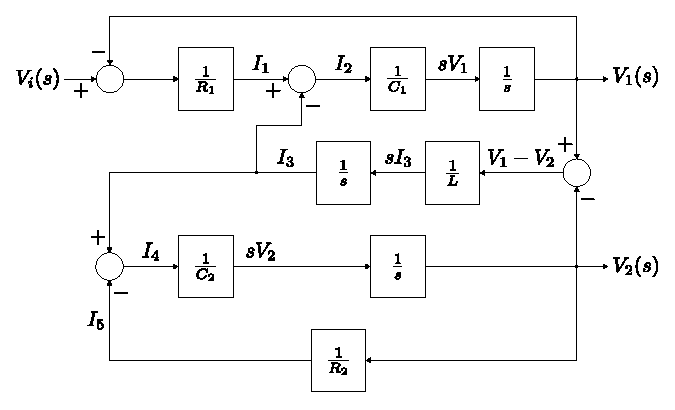
\includegraphics[width=\linewidth]{cap2_fig1.eps}
    \caption{Schéma fonctionnel.}
    \label{fig:exemple1}
\end{figure}
\end{verbatim}

Ce code produit Figure~\ref{fig: exemple1}. Les figures peuvent être redimensionnées à l'aide de l'option \code{scale}, ou relatives, par exemple, à la largeur de la zone de texte de la forme: \path{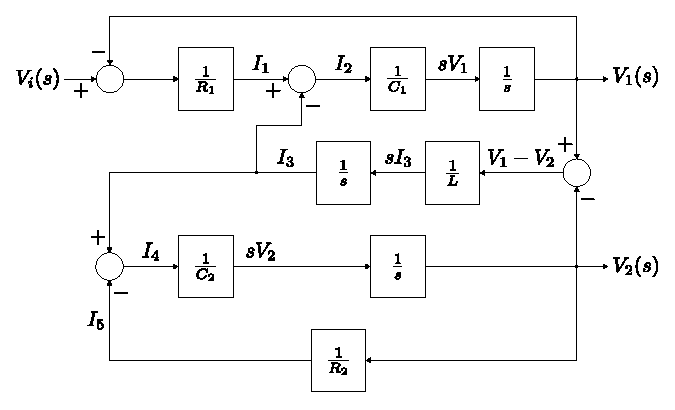
\includegraphics[width=0.5\textwidth]{cap2_fig1.eps}}. Si nécessaire, vous pouvez également utiliser des sous-figures (voir code dans ce fichier), comme le montre la Figure~\ref{fig: example2} qui contient les sous-figures~\ref{fig: subfigA} et~\ref{fig : subfigB}.

\begin{figure}[htbp]
    \center
    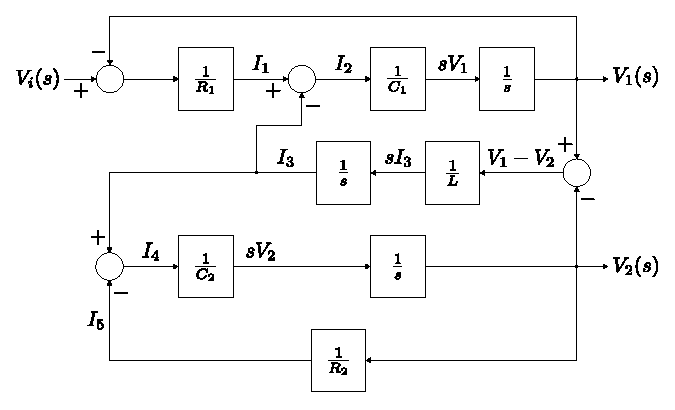
\includegraphics[scale=0.8]{cap2_fig1.eps}
    \caption{Schéma fonctionnel.}
    \label{fig:exemple1}
\end{figure}

\begin{figure} [htbp]
  \center
  \subcaptionbox{Une sous-figure \label{fig:subfigA}}{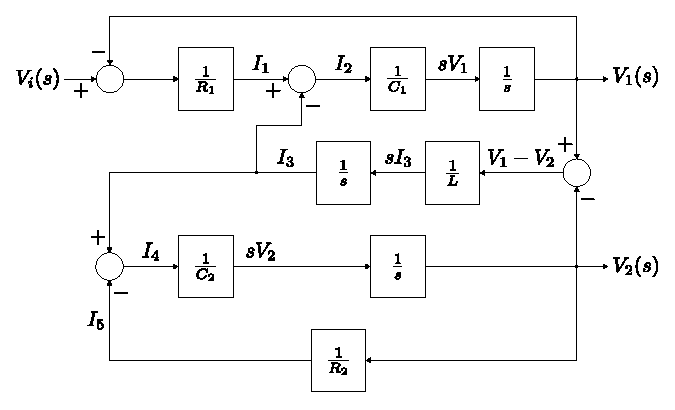
\includegraphics[width=0.45\linewidth]{cap2_fig1.eps}}
% \hfill
  \subcaptionbox{\label{fig:subfigB}}{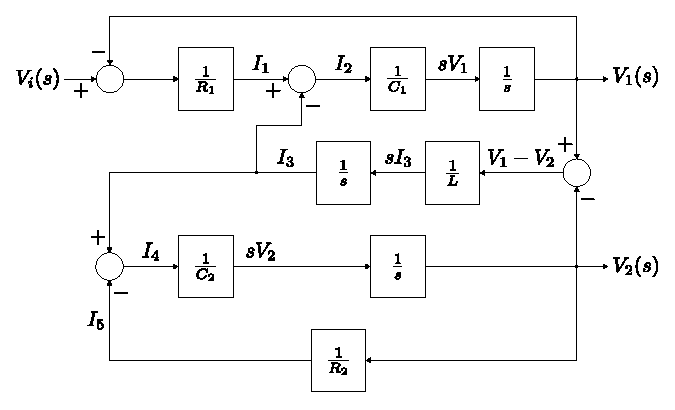
\includegraphics[width=0.45\linewidth]{cap2_fig1.eps}}
  \caption[Une figure avec deux sous-figures.]{Une figure avec deux sous-figures: (a) avec une légende et (b) sans une légende \cite{Motorola96}.}
  \label{fig:exemple2}
\end{figure}

Gardez à l'esprit que les chiffres n'apparaîtront pas toujours à l'endroit où vous avez écrit le code, car le placement dépend de l'espace disponible sur la page. Le positionnement des figures est un travail pour \LaTeX{} et vous ne devriez donc vous préoccuper que de la création d'images, de préférence au format vectoriel (par exemple, EPS, PDF). En ce sens, il existe plusieurs outils et Inkscape (\url{inkscape.org}) est une excellente alternative. \LaTeX{} accepte par défaut les formats PDF, JPG et PNG. Les figures doivent toujours être référencées dans le texte et doivent également toujours avoir une légende, définie à l'aide de la commande \verb|\caption{}|. N'oubliez pas que lorsqu'une figure est obtenue à partir d'une référence bibliographique, c'est-à-dire qu'elle n'est pas de son auteur, ce fait doit être mentionné (voir légende de la figure~\ref{fig:exemple2}).

Ce \textit{template} fournit la commande supplémentaire \verb|\inlinegraphics| qui vous permet d'insérer des figures dans la ligne de texte. Ceci est un exemple \inlinegraphics{Inlinefigureexample.png}, vérifiez comment utiliser la commande dans le code de ce fichier. Parfois, une figure doit être affichée dans \textit{paysage}, où Figure~\ref{fig:exemple3} est un exemple de cette forme de présentation.

%%%%%%%%%%%%%%%%%%%%%%%%%%%%%%%%%%%%

\paragraph{Tables}

Les tableaux sont un moyen important de présenter les informations. Le tableau~\ref{tab: basictable} illustre l'application des principales directives à prendre en compte lors de la construction des tableaux:

\begin{enumerate}
   \item N'utilisez pas de lignes verticales,
   \item La légende est placée avant le tableau,
   \item Utilisez les macros \verb|\toprule|, \verb|\midrule| e \verb|\bottomrule| pour créer respectivement les lignes horizontales du haut, du milieu et du bas du tableau.
\end{enumerate}

\begin{landscape}
    \begin{figure} [htbp]
        \center
        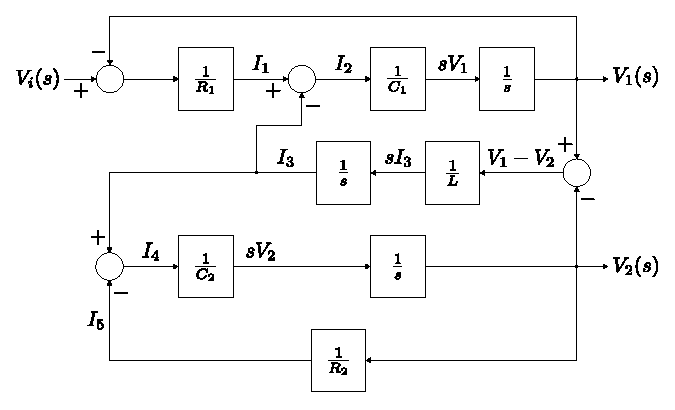
\includegraphics[width=0.8\linewidth]{cap2_fig1.eps}
        \caption{Une figure dans \textit{paysage}.}
        \label{fig:exemple3}
    \end{figure}
\end{landscape}

Considérez le code suivant utilisé pour créer la table~\ref{tab: basictable}:
{\small
\begin{verbatim}
\begin{table}
    \caption{Exemple de tableau simple dans \LaTeX{}.}
    \label{tab: basictable}
    \center
    \begin{tabular}{l c c}
        \toprule
        \tabhead{Colonne 1} & \tabhead{Colonne 2} & \tabhead{Colonne 3} \\
        \midrule
        Ligne 1 & 0,2 & 0,8 \\
        Ligne 2 & 0,17 & 0,7 \\
        Ligne 3 & 0,24 & 0,75 \\
        Ligne 4 & 0,68 & 0,3 \\
        \bottomrule
    \end{tabular}
\end{table}
\end{verbatim}
}

\begin{table}[htb]
    \caption{Exemple de tableau simple dans \LaTeX{}.}
    \label{tab:basictable}
    \center
    \begin{tabular}{l c c}
        \toprule
        \tabhead{Colonne 1} & \tabhead{Colonne 2} & \tabhead{Colonne 3} \\
        \midrule
        Ligne 1 & 0,2 & 0,8 \\
        Ligne 2 & 0,17 & 0,7 \\
        Ligne 3 & 0,24 & 0,75 \\
        Ligne 4 & 0,68 & 0,3 \\
        \bottomrule
    \end{tabular}
\end{table}

Pour faire référence aux tables, utilisez la commande \verb|\ref{<label>}|, où \verb|<label>| fait référence à l'étiquette définie par \verb|\label{<label>}|. En règle générale, mettez toujours un tilde, c'est-à-dire \verb|Table~\ref{<label>}|, pour introduire un \textit{espace incassable}. Des environnements et des commandes supplémentaires peuvent être utilisés pour créer des tables plus complexes/spécifiques (tant que les règles générales définies ci-dessus sont maintenues): \verb|tabularx|, \verb|longtable|, \verb|\multicolumn|, \verb|\multirow|, entre autres. En cas de difficulté dans la création du code des tables, \textit{website} \url{www.tablesgenerator.com} est suggéré.

%%%%%%%%%%%%%%%%%%%%%%%%%%%%%%%%%%%%

\paragraph{Listes de codes}

Pour afficher des extraits de code source dans votre rapport, ce \textit{template} utilise \gls{pack} \verb|listings|. Gardez à l'esprit que par défaut, les listes sont définies pour flotter afin que \LaTeX{} puisse les positionner de la meilleure façon. Cette définition implique également qu'une liste ne sera pas divisée par une nouvelle page, il est donc recommandé d'utiliser des extraits qui ne dépassent pas une page. Il existe de nombreuses options qui peuvent être spécifiées dans cet environnement, pour plus d'informations, voir \url{en.wikibooks.org/wiki/LaTeX/Source_Code_Listings}.

La commande \verb|\printlistoflistings|, invoquée dans le fichier \path{4_frontmatterlists.tex}, crée la section `` Listes '' dans votre document. Donc, si vous n'avez pas besoin d'utiliser des listes, vous devriez commenter cette commande. La liste~\ref{lst: examplo1} et la liste~\ref{lst: examplo2} sont deux exemples de listes de codes. Veuillez consulter le contenu de ce fichier pour plus de détails.

\begin{center}
    \begin{minipage}{0.7 \linewidth}
        \begin{lstlisting} [language=C, caption=Exemple simple de C., label=lst:examplo1]
        #include <stdio.h>
        main()
        {
        printf ("Bonjour le monde");
        }
        \end{lstlisting}
    \end{minipage}
\end{center}

Une liste de codes peut également être insérée directement à partir d'un fichier en utilisant la commande \verb|\lstinputlisting[<settings>]{<pathtofile>/file.c}|.

\begin{minipage}{0.9 \linewidth}
    \begin{lstlisting} [language=Python, caption=Exemple long en Python., label=lst:examplo2]
import numpy as np
    
def incmatrix(genl1,genl2):
    m = len(genl1)
    n = len(genl2)
    M = None #to become the incidence matrix
    VT = np.zeros((n*m,1), int)  #dummy variable
    
    #compute the bitwise xor matrix
    M1 = bitxormatrix(genl1)
    M2 = np.triu(bitxormatrix(genl2),1) 

    for i in range(m-1):
        for j in range(i+1, m):
            [r,c] = np.where(M2 == M1[i,j])
            for k in range(len(r)):
                VT[(i)*n + r[k]] = 1;
                VT[(i)*n + c[k]] = 1;
                VT[(j)*n + r[k]] = 1;
                VT[(j)*n + c[k]] = 1;
                
                if M is None:
                    M = np.copy(VT)
                else:
                    M = np.concatenate((M, VT), 1)               
                VT = np.zeros((n*m,1), int)  
    return M
    \end{lstlisting}
\end{minipage}

%%%%%%%%%%%%%%%%%%%%%%%%%%%%%%%%%%%%%%%%%%%%%%%%%%%%%%%%%%%%%%%%%%%%%%%%%%%%%%%%%%%%%%%%%%%%%%%%%%%%%%%

\paragraph{Équations}

Si votre thèse utilise un contenu mathématique, alors l'option d'utiliser \LaTeX{} était la bonne. Le livre ``Une pas si petite introduction à \LaTeX{}'' contient suffisamment d'informations pour la plupart des cas de composition mathématique, mais pour un contenu plus complet, le guide \url{tug.ctan.org/info/short est recommandé -math- guide / short-math-guide.pdf}. De plus, une liste complète de symboles peut être trouvée sur \url{tug.ctan.org/info/symbols/comprehensive/symbols-a4.pdf}.

\LaTeX{} vous permet d'écrire des équations \textit{inline} telles que $E = mc^{2}$ ou en mode \textit{display}, auquel cas elles sont automatiquement numérotées:
\begin{verbatim}
\begin{equation}
    E=mc^{2}.
    \label{eqn:einstein}
\end{equation}
\end{verbatim}

\noindent qui produit la fameuse équation:
\begin{equation}
    E=mc^{2}.
    \label{eqn:einstein}
\end{equation}

Alternativement, si vous voulez que (\ref{eqn:einstein}) ne soit pas numéroté, vous pouvez utiliser le code \verb|$$E=mc^{2}$$| qui produit:
$$E=mc ^{2}.$$

%%%%%%%%%%%%%%%%%%%%%%%%%%%%%%%%%%%%%%%%%%%%%%%%%%%%%%%%%%%%%%%%%%%%%%%%%%%%%%%%%%%%%%%%%%%%%%%%%%%%%%%

\paragraph{Théorèmes}

Les théorèmes, les lemmes et les corollaires doivent être numérotés par ordre croissant. Le \textit{template} fournit ces environnements adaptés à la langue sélectionnée pour le document dans \file{main.tex}. Via la commande \verb|\newtheorem| vous pouvez créer des environnements supplémentaires du même type (dans le fichier \file{preamble.tex}).

\begin{theorem}
Ceci est un exemple d'application de l'environnement \code{theorem}. Les théorèmes sont numérotés par ordre croissant, à partir de 1.
\end{theorem}

\begin{corollary}
Ceci est un exemple de l'application de l'environnement \code{corollary}. Les corollaires sont numérotés par ordre croissant, à partir de 1.
\end{corollary}

\begin{lemma}
Voici un exemple d'application de l'environnement \code{lemma}. Les devises sont numérotées par ordre croissant, à partir de 1.
\end{lemma}

%%%%%%%%%%%%%%%%%%%%%%%%%%%%%%%%%%%%%%%%%%%%%%%%%%%%%%%%%%%%%%%%%%%%%%%%%%%%%%%%%%%%%%%%%%%%%%%%%%%%%%%
\clearpage
\section{Notes supplémentaires}

\textbf{Bonne chance!}		
%%%%%%%%%%%%%%%%%%%%%%%%%%%%%%%%%%%% Chapter Template

\chapter{Conclusion} 	% Main chapter title
\label{Chapter6} 		% For referencing the chapter elsewhere, usage \ref{Chapter6}

%%%%%%%%%%%%%%%%%%%%%%%%%%%%%%%%%%%%

\lipsum[1]

%%%%%%%%%%%%%%%%%%%%%%%%%%%%%%%%%%%%

\section{Perspectives}
\label{sec:Ch6.1}

\lipsum[1] 



%%%%%%%%%%%%%%%%%%%%%%%%%%%%%%%%%%%%%%%%%%%%%%%%%%%%%%%%%%%%%%%%%%%%%%%%%%%%%%%%%%%%%%%%%
% Print the bibliographic references using the ieeetr format from the 'sampleRefs.bib' file (root folder)

\printrefereces{sampleRefs}		% Change the 'sampleRefs' name to match your .bib file name,
								% a good option to make bib files is https://www.jabref.org/
%%%%%%%%%%%%%%%%%%%%%%%%%%%%%%%%%%%%%%%%%%%%%%%%%%%%%%%%%%%%%%%%%%%%%%%%%%%%%%%%%%%%%%%%%
\appendix
% Include the appendices of the document as separate files from the 'chapters' folder
% Fiche nº1

\chapter{Fiche nº1} % Main appendix title
\label{app:Fiche1} % For referencing this appendix elsewhere, use \ref{app:Fiche1}

%%%%%%%%%%%%%%%%%%%%%%%%%%%%%%%%%%%%%%%%%%%%%%%%%%%%%%%%%%%%%%%%%%%%%%%%%%%%%%%%%%
\section{Description de l'article}

\paragraph{Titre de l'article~: Correlating the effects of flow and telepresence in virtual worlds: Enhancing
our understanding of user behavior in game-based learning}
\paragraph{Lien de l'article~:}
\paragraph{Liste des auteurs~: Anthony Faiola (a), Christine Newlon (a), Mark Pfaff (a), Olga Smyslova (b)}
\paragraph{Affiliation des auteurs~: (a) Indiana University, School of Informatics (IUPUI), Indianapolis, IN, USA.
(b) Kaiser Permanente, USA}
\paragraph{Nom de la conférence / revue~: Computers in Human Behavior 29 (2013)}
\paragraph{Classification de la conférence / revue~: H-Index 251 (scimagojr.com)}
\paragraph{Nombre de citations de l'article (quelle source ?)~: 329 (Google Scholar)}



%%%%%%%%%%%%%%%%%%%%%%%%%%%%%%%%%%%%%%%%%%%%%%%%%%%%%%%%%%%%%%%%%%%%%%%%%%%%%%%%%%
\section{Synthèse de l'article}

\paragraph{Problématique}

Blabla

\paragraph{Pistes possibles (pointés par les auteurs)}
\lipsum[1]

\paragraph{Question de recherche}
\lipsum[1]

\paragraph{Démarche adoptée}
\lipsum[1]

\paragraph{Implémentation de la démarche}
\lipsum[1]

\paragraph{Les résultats}
\lipsum[1]
	% Uncomment the lines as you write the summaries,
% Fiche nº2

\chapter{Fiche nº2} % Main appendix title
\label{app:Fiche2} % For referencing this appendix elsewhere, use \ref{app:Fiche2}

%%%%%%%%%%%%%%%%%%%%%%%%%%%%%%%%%%%%%%%%%%%%%%%%%%%%%%%%%%%%%%%%%%%%%%%%%%%%%%%%%%
\section{Description de l'article}

\paragraph{Titre de l'article~:}
\paragraph{Lien de l'article~:}
\paragraph{Liste des auteurs~:}
\paragraph{Affiliation des auteurs~:}
\paragraph{Nom de la conférence / revue~:}
\paragraph{Classification de la conférence / revue~:}
\paragraph{Nombre de citations de l'article (quelle source ?)~:}



%%%%%%%%%%%%%%%%%%%%%%%%%%%%%%%%%%%%%%%%%%%%%%%%%%%%%%%%%%%%%%%%%%%%%%%%%%%%%%%%%%
\section{Synthèse de l'article}

\paragraph{Problématique}
\lipsum[1]

\paragraph{Pistes possibles (pointés par les auteurs)}
\lipsum[1]

\paragraph{Question de recherche}
\lipsum[1]

\paragraph{Démarche adoptée}
\lipsum[1]

\paragraph{Implémentation de la démarche}
\lipsum[1]

\paragraph{Les résultats}
\lipsum[1]
	% Uncomment the lines as you write the summaries,
% Fiche nº3

\chapter{Fiche nº3} % Main appendix title
\label{app:Fiche3} % For referencing this appendix elsewhere, use \ref{app:Fiche3}

%%%%%%%%%%%%%%%%%%%%%%%%%%%%%%%%%%%%%%%%%%%%%%%%%%%%%%%%%%%%%%%%%%%%%%%%%%%%%%%%%%
\section{Description de l'article}

\paragraph{Titre de l'article~:}
\paragraph{Lien de l'article~:}
\paragraph{Liste des auteurs~:}
\paragraph{Affiliation des auteurs~:}
\paragraph{Nom de la conférence / revue~:}
\paragraph{Classification de la conférence / revue~:}
\paragraph{Nombre de citations de l'article (quelle source ?)~:}



%%%%%%%%%%%%%%%%%%%%%%%%%%%%%%%%%%%%%%%%%%%%%%%%%%%%%%%%%%%%%%%%%%%%%%%%%%%%%%%%%%
\section{Synthèse de l'article}

\paragraph{Problématique}

Les recherches sur l'apprentissage en VR semblent se concentrer sur une comparaison des médias par lesquels passe l'apprentissage,
plutôt que sur les facteurs humains qui guident l'apprentissage.

\paragraph{Pistes possibles (pointés par les auteurs)}

La négligeance des ressentis de l'utilisateur dans son environnement d'apprentissage représente un obstacle dans les objectifs d'apprentissage

\paragraph{Question de recherche}

Quels sont les réels impacts de l'immersion et de l'intéractivité en VR sur les capacités d'apprentissage.

\paragraph{Démarche adoptée}

Regarder les impacts isolés des notions d'intéractivité et d'immersion,
tester le framework CAMIL

\paragraph{Implémentation de la démarche}

Expérience où une leçon sera instruite à travers différents média à l'immersion et à l'interactivité diverses (vidéo,PC, VR-video, VR)
(Ici l'immersion est surtout visuelle)
180 participants adultes, 153 données ont été analysées.

Creation d'un musée virtuel sur le sujet de maladies virologiques
2 versions: une visite pré-enregistrée (interactivité basse), une visite libre (interactivité haute)
Tester empiriquement les hypothèses présentées par le framework CAMIL en utilisant une modélisation d'équation structurelle (SEM)


\paragraph{Les résultats}
\lipsum[1]

Hypothesis of CAMIL on VR learning
"the path from VR features to learning outcomes was mediated by non-cognitive outcomes such as motivation, presence, and usability"


both interactivity and immersion were shown to impact agency, physical presence, and embodied learning positively

Although interactivity still influenced agency and embodied learning when lessons were highly immersive, the impact was not as strong as when the lesson was less immersive. Supposedly, being visually immersed is such a powerful experience in itself that interactivity provides less added value; under conditions of low visual immersion, however, interactivity is shown to its full advantage

No effects of interactivity or immersion on intrinsic motivation, self-efficacy, extraneous cognitive load interaction, or learning were found.	% Uncomment the lines as you write the summaries,
% Fiche nº4

\chapter{Fiche nº4} % Main appendix title
\label{app:Fiche4} % For referencing this appendix elsewhere, use \ref{app:Fiche4}

%%%%%%%%%%%%%%%%%%%%%%%%%%%%%%%%%%%%%%%%%%%%%%%%%%%%%%%%%%%%%%%%%%%%%%%%%%%%%%%%%%
\section{Description de l'article}

\paragraph{Titre de l'article~:}
\paragraph{Lien de l'article~:}
\paragraph{Liste des auteurs~:}
\paragraph{Affiliation des auteurs~:}
\paragraph{Nom de la conférence / revue~:}
\paragraph{Classification de la conférence / revue~:}
\paragraph{Nombre de citations de l'article (quelle source ?)~:}



%%%%%%%%%%%%%%%%%%%%%%%%%%%%%%%%%%%%%%%%%%%%%%%%%%%%%%%%%%%%%%%%%%%%%%%%%%%%%%%%%%
\section{Synthèse de l'article}

\paragraph{Problématique}
\lipsum[1]

\paragraph{Pistes possibles (pointés par les auteurs)}
\lipsum[1]

\paragraph{Question de recherche}
\lipsum[1]

\paragraph{Démarche adoptée}
\lipsum[1]

\paragraph{Implémentation de la démarche}
\lipsum[1]

\paragraph{Les résultats}
\lipsum[1]
	% Uncomment the lines as you write the summaries,

% Appendix A

\chapter{Titre de l'annexe} % Main appendix title
\label{AppendixA} % For referencing this appendix elsewhere, use \ref{AppendixA}

%%%%%%%%%%%%%%%%%%%%%%%%%%%%%%%%%%%%%%%%%%%%%%%%%%%%%%%%%%%%%%%%%%%%%%%%%%%%%%%%%%
\section{Section}

\lipsum[1]

%%%%%%%%%%%%%%%%%%%%%%%%%%%%%%%%%%%%%%%%%%%%%%%%%%%%%%%%%%%%%%%%%%%%%%%%%%%%%%%%%%
\section{Une autre section de l'annexe~\ref{AppendixA}}

\lipsum[1]

	% Uncomment the lines as you write the appendices,
%\include{chapters/appendixB}	% or comment the lines if not used

%%%%%%%%%%%%%%%%%%%%%%%%%%%%%%%%%%%%%%%%%%%%%%%%%%%%%%%%%%%%%%%%%%%%%%%%%%%%%%%%%%%%%%%%%
\end{document}  
